%!TEX root = ./template-skripsi.tex
%-------------------------------------------------------------------------------
%                            	BAB IV
%               		KESIMPULAN DAN SARAN
%-------------------------------------------------------------------------------

\chapter{UJI COBA DAN HASIL UJI COBA}

\section{Uji Coba}
Uji coba sistem dilakukan terhadap 30 responden anggota KOPMA UNJ dengan rincian, \textit{admin} yang terdiri dari 2 responden, pengawas yang terdiri dari 3 responden, dan anggota yang terdiri dari 25 responden. Setiap responden akan melakukan uji coba terhadap sistem yang dibuat berdasarkan peran masing-masing responden. Uji coba yang dilakukan menggunakan data dari hasil sebaran kuesioner \textit{User Acceptance Test}. \textit{User Acceptance Test} bertujuan untuk mengetahui perihal sistem yang dikembangkan apakah sudah sesuai dengan kebutuhan \textit{user} atau belum. Skala yang digunakan dalam penelitian ini adalah skala \textit{likert}.

Langkah-langkah pengujian sistem informasi Koperasi Mahasiswa Universitas Negeri Jakarta yang akan dilakukan adalah sebagai berikut:
\begin{enumerate}
	\item \textit{User} melakukan pendaftaran anggota.
	\item \textit{Admin} melakukan verifikasi penerimaan anggota.
	\item \textit Seluruh \textit{user} dapat mengelola biodata pribadi.
	\item \textit{Admin} mengelola status keanggotaan setiap \textit{user} (\textit{admin}, pengawas, atau anggota biasa).
	\item Anggota dan pengawas yang sudah memiliki akun dapat mengakses ke dalam sistem sesuai berandanya masing-masing.
	\item \textit{Admin} menambahkan data barang, stok, simpanan, transaksi anggota, dan keuangan.
	\item Data yang \textit{admin} tambahkan akan muncul dan dapat dilihat di beranda semua \textit{user}.
	\item \textit{Admin} mengelola (sunting dan hapus) data barang, stok, simpanan, transaksi anggota, dan keuangan.
	\item Data yang \textit{admin} kelola akan berubah dan dapat dilihat di beranda semua \textit{user}.	
	\item Pengawas menambahkan data penilaian untuk KOPMA UNJ.
	\item Data yang pengawas tambahkan akan muncul dan dapat dilihat di beranda  semua \textit{user}.
	\item Pengawas mengelola (sunting dan hapus) data penilaian untuk KOPMA UNJ.
	\item Data yang pengawas kelola akan berubah dan dapat dilihat di beranda semua \textit{user}.	
\end{enumerate}

Fitur milik setiap \textit{user} yang akan diuji pada sistem informasi Koperasi Mahasiswa Universitas Negeri Jakarta adalah sebagai berikut:

\begin{itemize}
	\item \textit{Admin}
	\begin{enumerate}
		\item Masuk ke dalam sistem
		\item Penyuntingan data pribadi
		\item Pengelolaan anggota (tambah, kesesuaian \textit{id}, detail, pemutihan, sunting, \textit{reset password}, tambah periode, pengelompokan, pemulihan, keuangan anggota, dan cetak)
		\item Pengelolaan barang (tambah, sunting, hapus, cetak, dan pengelompokan)
		\item Pengelolaan stok (tambah, hapus, dan cetak)
		\item Pengelolaan simpanan (tambah, hapus, cetak, dan pengelompokan)
		\item Pengelolaan transaksi (tambah, hapus, dan cetak)
		\item Transparansi penilaian
		\item Pengelolaan dan kesesuaian arus keuangan (tambah dana tambahan dan beban lain)
		\item Pengelolaan \textit{admin} (tambah dan hapus \textit{admin})
		\item Pengelolaan pengawas (tambah dan hapus pengawas)
		\item Pengelolaan penerimaan anggota (terima dan tolak anggota)
		\item Keluar dari sistem
	\end{enumerate}

	\item Anggota
	\begin{enumerate}
		\item Melakukan pendaftaran
		\item Masuk ke dalam sistem
		\item Penyuntingan data pribadi
		\item Transparansi data (barang, stok, transaksi, penilaian, dan arus keuangan)
		\item Keluar dari sistem
	\end{enumerate}
	
	\item Pengawas
	\begin{enumerate}
		\item Masuk ke dalam sistem
		\item Penyuntingan data pribadi
		\item Transparansi data (barang, stok, transaksi, dan arus keuangan)
		\item Pengelolaan penilaian (tambah, sunting, hapus, dan cetak)
		\item Keluar dari sistem
		\end{enumerate}
	\end{itemize}

Semua fitur yang diuji memiliki penilaian yang dirincikan menjadi beberapa kategori. Data kuantitatif akan dianalisis dengan menggunakan skala \textit{ likert}. Berikut kategori dan skor penilaian dalam tahap pengujian\textit{ User Acceptance Test} pada sistem informasi Koperasi Mahasiswa Universitas Negeri Jakarta dengan menggunakan skala \textit{likert}:\\

\begin{tabular}{lll}
SS& = Sangat Setuju& diberikan nilai 5\\
S& = Setuju& diberikan nilai 4\\
C& = Cukup& diberikan nilai 3\\
TS& = Tidak Setuju& diberikan nilai 2\\
STS& = Sangat Tidak Setuju& diberikan nilai 1\\
\\
\end{tabular}

Kemudian hasil pendataan yang telah didapatkan dengan teknik penyebaran angket dikalkulasikan dengan menggunakan sistem penilaian sebagai berikut:

\begin{itemize}
	\item Nilai total
	
	Nilai total merupakan nilai dari hasil perhitungan antara responden kuesioner angket dengan nilai di setiap poin pertanyaan. Berikut merupakan rumus nilai total:
	
	\textit{Nilai total = jumlah nilai setiap soal}
	
	\item Nilai rata-rata
	
	Nilai rata-rata merupakan nilai dari hasil perhitungan antara nilai total dengan jumlah responden yang mengisi kuesioner angket. Berikut merupakan rumus dari nilai rata-rata:

	\textit{Nilai rata-rata = nilai total / jumlah responden}
	
\end{itemize}

Untuk mengetahui kualitas produk yang dikembangkan layak atau tidak, maka perlu ditentukan dengan menghitung seluruh nilai rata-rata dari setiap pertanyaan. Nilai tersebut kemudian akan dibandingkan dengan interpretasi skor pada skala \textit{likert}. Analisis data yang disajikan ke distribusi skor dan persentase terhadap kategori menggunakan interpretasi skor untuk skala \textit{likert}. Berikut rentang interpretasi skor untuk skala \textit{likert}:\\

\begin{tabular}{lll}
	Nilai& = 0\% - 20\%& Sangat Kurang Sesuai \\
	Nilai& = 21\% - 40\%& Kurang Sesuai\\
	Nilai& = 41\% - 60\%& Cukup Sesuai\\
	Nilai& = 61\% - 80\%& Sesuai\\
	Nilai& = 81\% - 100\%& Sangat Sesuai\\
\end{tabular}

\section{Hasil Uji Coba}
Berdasarkan hasil uji coba \textit{User Acceptance Test} yang dilakukan terhadap 30 anggota KOPMA UNJ, yakni \textit{admin} yang terdiri dari 2 responden, pengawas terdiri dari 3 responden, dan anggota terdiri dari 25 responden, diperoleh hasil uji coba sebagai berikut:

\subsection{\textit{Admin}}
Berikut merupakan daftar pertanyaan \textit{User Acceptance Test} pada \textit{Admin}:

\begin{table}[H]
	\centering
	\caption{Daftar Pertanyaan \textit{User Acceptance Test} pada \textit{Admin}}
	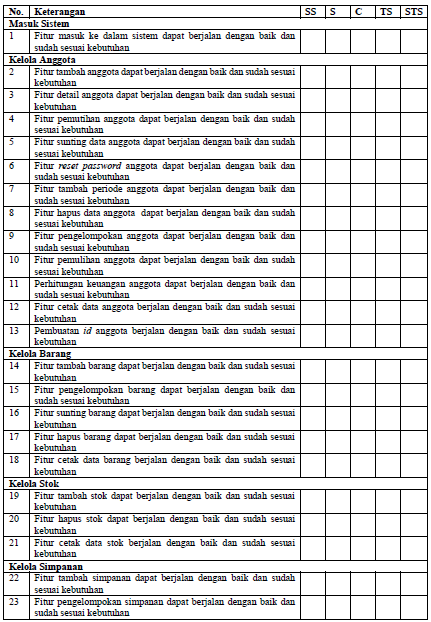
\includegraphics[width=1.0\textwidth]{gambar/Tabel_Admin1}
\end{table}

\begin{table}[H]
	\centering
	\caption{Daftar Pertanyaan \textit{User Acceptance Test} pada \textit{Admin}}
	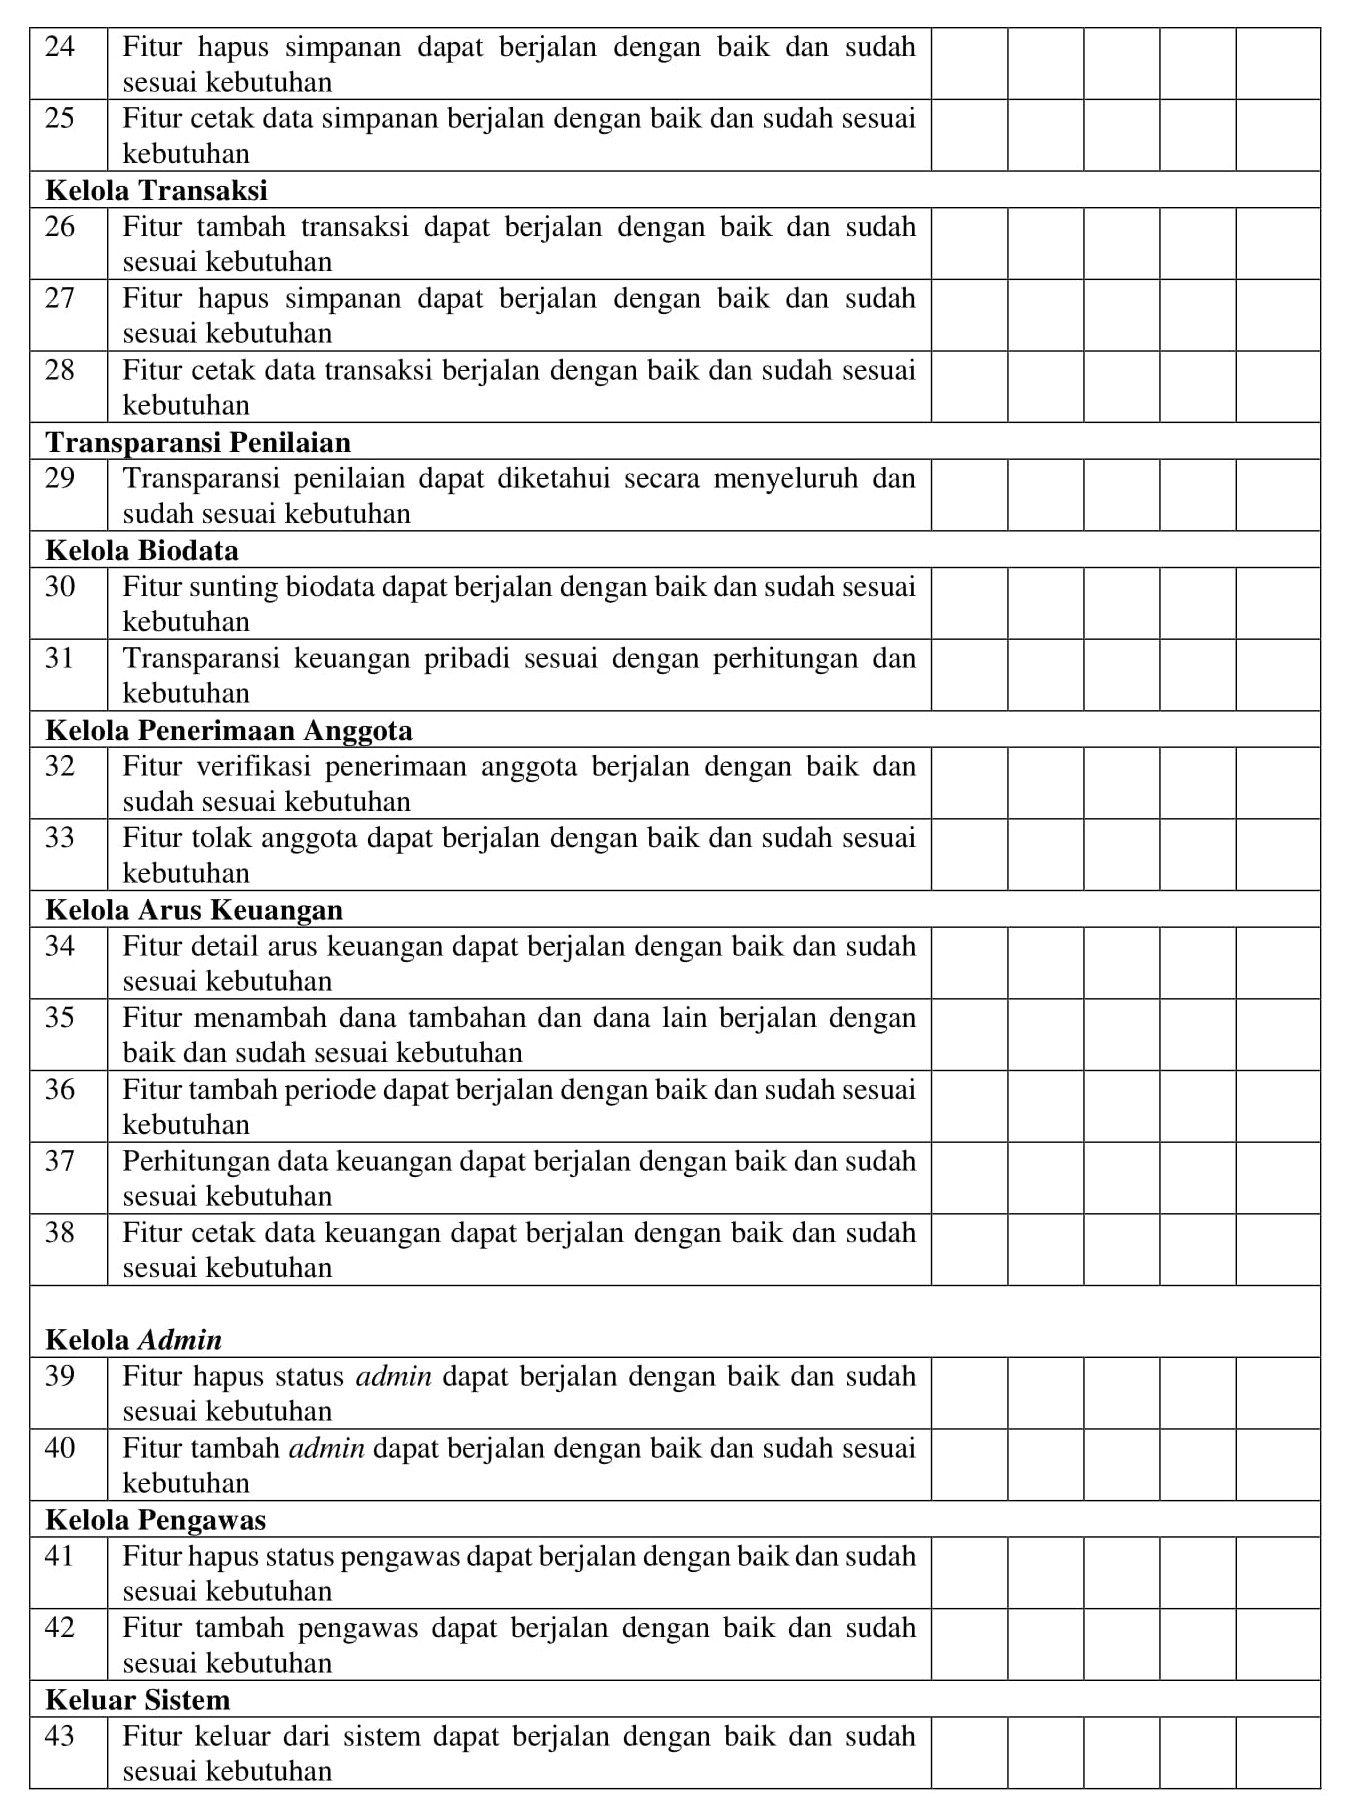
\includegraphics[width=1.0\textwidth]{gambar/Tabel_Admin2}
\end{table}

Setelah kuisioner \textit{admin} diberikan kepada responden, kemudian data kuesioner diolah untuk mendapatkan hasil penilaian \textit{user acceptance test}. Adapun hasil penilaian \textit{user acceptance test} tersebut yaitu:

\begin{table}[H]
	\centering
	\caption{Data Hasil Penyebaran Kuesioner \textit{User Acceptance Test} pada \textit{Admin}}
	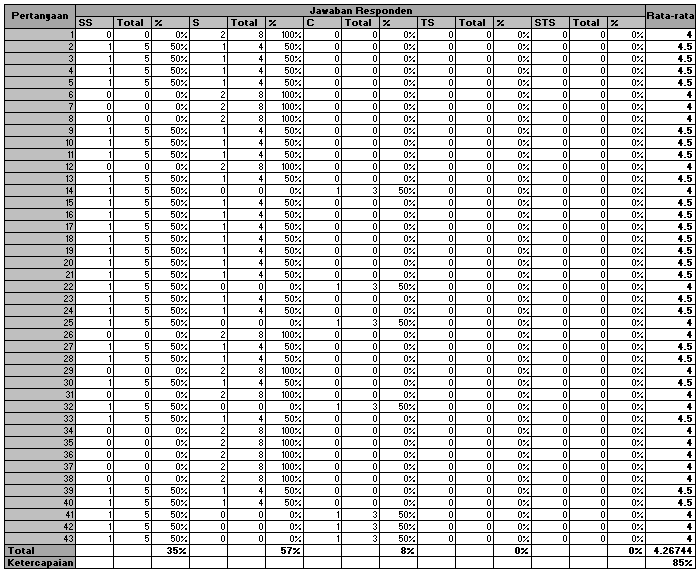
\includegraphics[width=1\textwidth]{gambar/Hasil_Admin}
\end{table}

Dari hasil penilaian pengujian \textit{user acceptance test} dapat diambil kesimpulan yaitu:

\begin{enumerate}
	\item Pengguna sistem yang telah memilih Sangat Tidak Setuju (STS) memiliki persentase 0\%
	\item Pengguna sistem yang telah memilih Tidak Setuju (TS) memiliki persentase 0\%
	\item Pengguna sistem yang telah memilih Cukup (C) memiliki persentase 8\%.
	\item Pengguna sistem yang telah memilih Setuju (S) memiliki persentase 57\%.
	\item Pengguna sistem yang telah memilih Sangat Setuju (SS) memiliki persentase 35\%.
	\item Rata-rata penerimaan \textit{user} adalah 4,27 dari 5 atau sekitar 85\%.
\end{enumerate}

\begin{figure}[H]
	\centering
	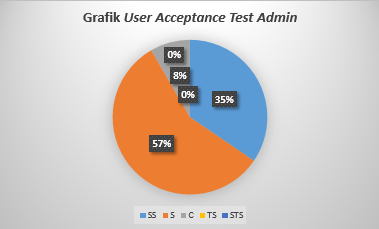
\includegraphics[width=1\textwidth]{gambar/Grafik_Admin}
	\caption{Grafik Hasil Penyebaran Kuesioner \textit{User Acceptance Test} pada \textit{Admin}}
\end{figure}

Berdasarkan hasil pengujian \textit{user acceptance test} yang diujikan kepada 2 responden \textit{admin}, dapat dilihat bahwa secara keseluruhan 35\% menjawab sangat setuju, 57\% menjawab setuju, 8\% menjawab cukup, serta rata-rata penerimaan \textit{user} terhadap kesesuaian sistem dengan kebutuhan adalah 4,27 dari 5 atau sekitar 85\%, oleh karena itu dapat diambil kesimpulan bahwa fitur yang \textit{admin} butuhkan dalam sistem informasi yang dirancang sudah sangat sesuai dengan kebutuhan dan berjalan dengan baik.  

\subsection{\textit{Anggota}}
Berikut merupakan daftar pertanyaan \textit{User Acceptance Test} pada Anggota

\begin{table}[H]
	\centering
	\caption{Daftar Pertanyaan \textit{User Acceptance Test} pada Anggota}
	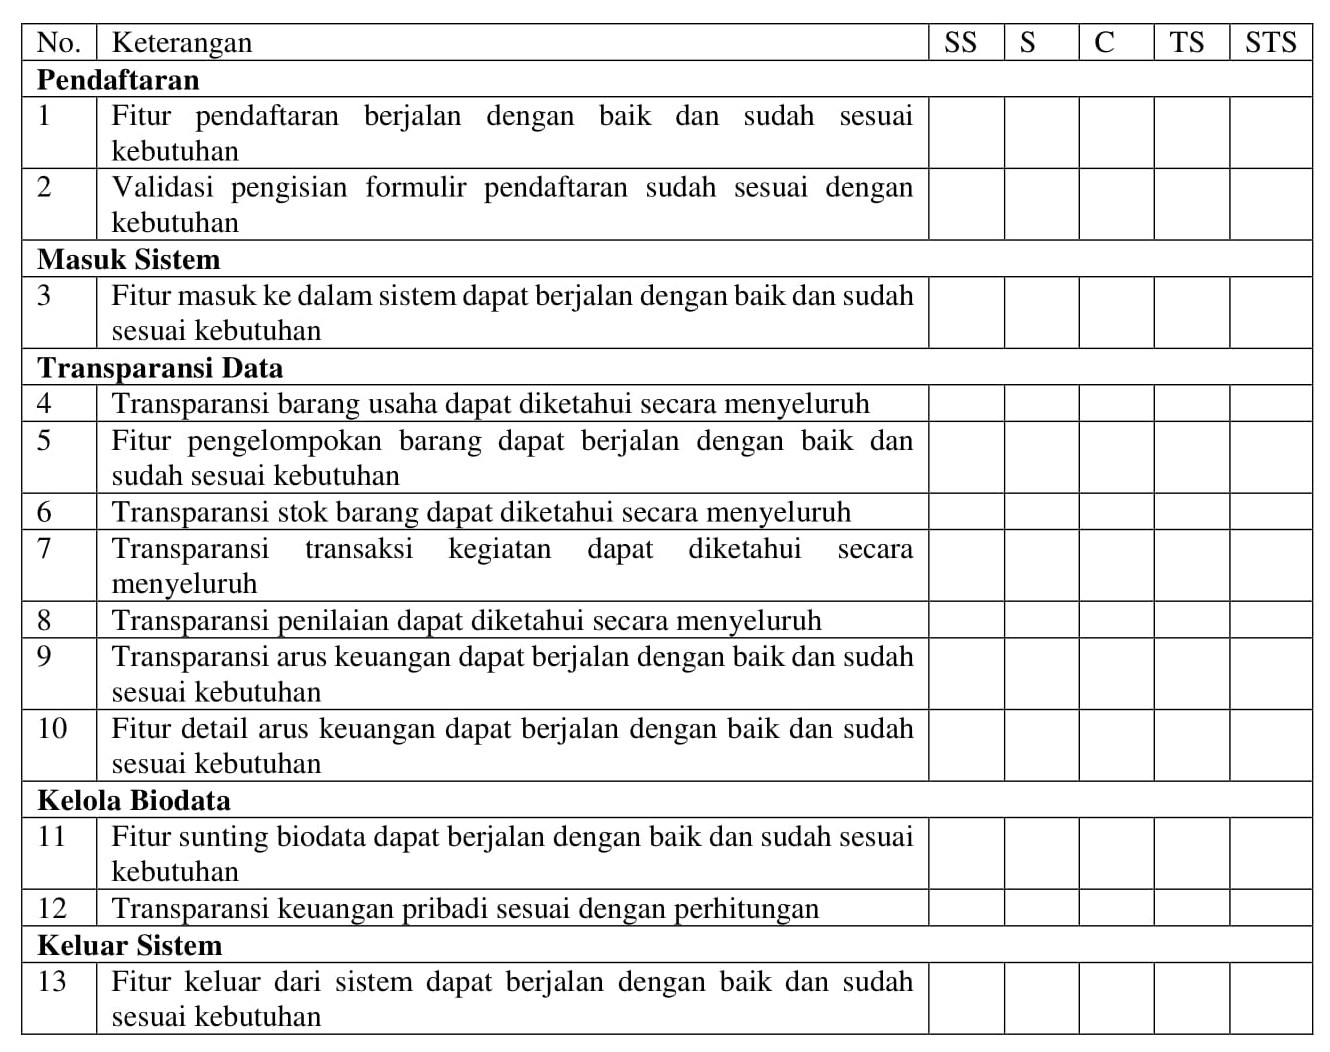
\includegraphics[width=1\textwidth]{gambar/Tabel_Anggota}
\end{table}

Setelah kuisioner anggota diberikan kepada responden, kemudian data kuesioner diolah untuk mendapatkan hasil penilaian \textit{user acceptance test}. Adapun hasil penilaian \textit{user acceptance test} tersebut yaitu:

\begin{table}[H]
	\centering
	\caption{Data Hasil Penyebaran Kuesioner \textit{User Acceptance Test} pada Anggota}
	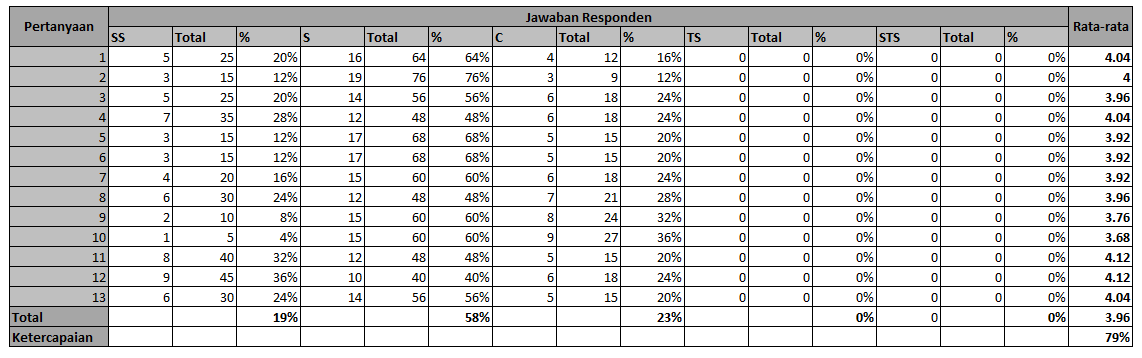
\includegraphics[width=1\textwidth]{gambar/Hasil_Anggota}
\end{table}

Dari hasil pengujian \textit{user acceptance test} dapat diambil kesimpulan yaitu:

\begin{enumerate}
	\item Pengguna sistem yang telah memilih Sangat Tidak Setuju (STS) memiliki persentase 0\%
	\item Pengguna sistem yang telah memilih Tidak Setuju (TS) memiliki persentase 0\%
	\item Pengguna sistem yang telah memilih Cukup (C) memiliki persentase 23\%.
	\item Pengguna sistem yang telah memilih Setuju (S) memiliki persentase 58\%.
	\item Pengguna sistem yang telah memilih Sangat Setuju (SS) memiliki persentase 19\%.
	\item Rata-rata penerimaan \textit{user} adalah 3,96 dari 5 atau sekitar 79\%.
\end{enumerate}

\begin{figure}[H]
	\centering
	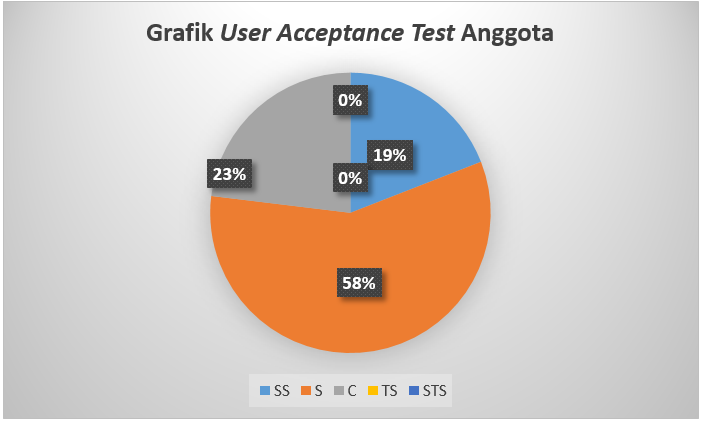
\includegraphics[width=1\textwidth]{gambar/Grafik_Anggota}
	\caption{Grafik Hasil Penyebaran Kuesioner \textit{User Acceptance Test} pada Anggota}
\end{figure}

Berdasarkan hasil pengujian \textit{user acceptance test} yang diujikan kepada 25 responden anggota, dapat dilihat bahwa secara keseluruhan 19\% menjawab sangat setuju, 58\% menjawab setuju, 23\% menjawab cukup, serta rata-rata penerimaan \textit{user} terhadap kesesuaian sistem dengan kebutuhan adalah 3,96 dari 5 atau sekitar 79\%, oleh karena itu dapat diambil kesimpulan bahwa fitur yang anggota butuhkan dalam sistem informasi yang dirancang sudah sesuai dengan kebutuhan dan berjalan dengan baik. 
\\
\\
\\
\\
\\

\subsection{\textit{Pengawas}}
Berikut merupakan daftar pertanyaan \textit{User Acceptance Test} pada Pengawas

\begin{table}[H]
	\centering
	\caption{Daftar Pertanyaan \textit{User Acceptance Test} pada Pengawas}
	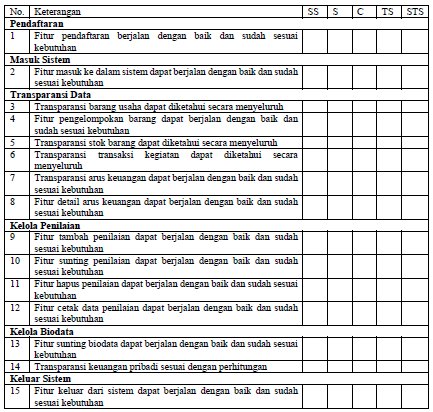
\includegraphics[width=1\textwidth]{gambar/Tabel_Pengawas}
\end{table}

Setelah kuisioner pengawas diberikan kepada responden, kemudian data kuesioner diolah untuk mendapatkan hasil penilaian \textit{user acceptance test}. Adapun hasil penilaian \textit{user acceptance test tersebut} tersebut yaitu:

\begin{table}[H]
	\centering
	\caption{Data Hasil Penyebaran Kuesioner \textit{User Acceptance Test} pada Pengawas}
	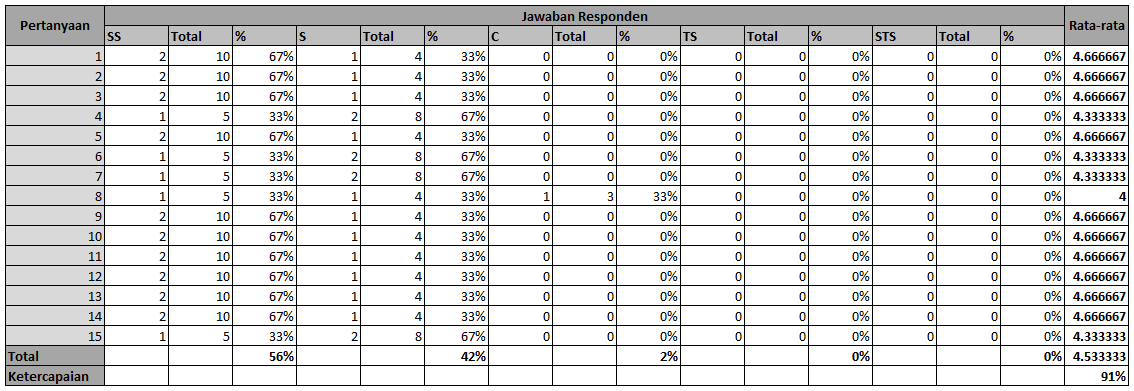
\includegraphics[width=1\textwidth]{gambar/Hasil_Pengawas}
\end{table}

Dari hasil penilaian pengujian \textit{user acceptance test} dapat diambil kesimpulan yaitu:

\begin{enumerate}
	\item Pengguna sistem yang telah memilih Sangat Tidak Setuju (STS) memiliki persentase 0\%
	\item Pengguna sistem yang telah memilih Tidak Setuju (TS) memiliki persentase 0\%
	\item Pengguna sistem yang telah memilih Cukup (C) memiliki persentase 2\%.
	\item Pengguna sistem yang telah memilih Setuju (S) memiliki persentase 42\%.
	\item Pengguna sistem yang telah memilih Sangat Setuju (SS) memiliki persentase 56\%.
	\item Rata-rata penerimaan \textit{user} adalah 4,53 dari 5 atau sekitar 91\%.
\end{enumerate}

\begin{figure}[H]
	\centering
	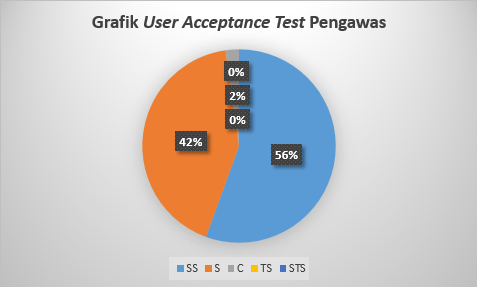
\includegraphics[width=1\textwidth]{gambar/Grafik_Pengawas}
	\caption{Grafik Hasil Penyebaran Kuesioner \textit{User Acceptance Test} pada Pengawas}
\end{figure}

Berdasarkan hasil pengujian \textit{user acceptance test} yang diujikan kepada 3 responden pengawas, dapat dilihat bahwa secara keseluruhan 56\% menjawab sangat setuju, 42\% menjawab setuju, 2\% menjawab cukup, serta rata-rata penerimaan \textit{user} terhadap kesesuaian sistem dengan kebutuhan adalah 4,53 dari 5 atau sekitar 91\%, oleh karena itu dapat diambil kesimpulan bahwa fitur yang pengawas butuhkan dalam sistem informasi yang dirancang sudah sangat sesuai dengan kebutuhan dan berjalan dengan baik. 

% Baris ini digunakan untuk membantu dalam melakukan sitasi
% Karena diapit dengan comment, maka baris ini akan diabaikan
% oleh compiler LaTeX.
\begin{comment}
\bibliography{daftar-pustaka}
\end{comment}